\documentclass[pdftex,12pt,a4paper]{report}

\usepackage[portuguese,english]{babel}
\usepackage[T1]{fontenc} 
\usepackage[utf8]{inputenc}
\usepackage[pdftex]{graphicx}
\usepackage{minitoc}
\usepackage{hyperref}
\usepackage{indentfirst}
\usepackage[compact]{titlesec}
\usepackage{fancyhdr}
\usepackage{caption}
\usepackage{pgfplots}
\usepackage{pgfplotstable}
\usepackage{fixltx2e}
\usepackage{mathtools}
\usepackage{fancyhdr}
\usepackage{listings}
\usepackage{color}
\usepackage{sverb}
\usepackage[section]{placeins}

%Highlight
\newcommand{\shellcmd}[1]{\indent\indent\texttt{\footnotesize\# #1}\\}

\pagestyle{fancy}
\renewcommand*\thesection{\thechapter\arabic{section}}
\newcommand{\HRule}{\rule{\linewidth}{0.5mm}}
\begin{document}

\begin{titlepage}

\begin{center}


\includegraphics[width=0.15\textwidth]{./logo}\\[0.5cm]    

\textsc{\large Universidade de Aveiro \\[1cm]\large departamento de electrónica, telecomunicações e informática}\\[1cm]

\textsc{\large{1}\large - Desempenho e Dimensionamento de Redes\\[1cm]}

\HRule \\[0.5cm]
{ \huge \bfseries abs}\\[0.4cm]
{ \large \bfseries x}\\[0.4cm]
\HRule \\[1cm]

\textsc{\small{8240 - MESTRADO INTEGRADO EM ENGENHARIA DE COMPUTADORES E TELEMÁTICA}}\\[1cm]

\begin{minipage}{0.4\textwidth}

\begin{flushleft} \large
\href{mailto:rafael.ferreira@ua.pt}{António Rafael da \\ Costa Ferreira }
 \small{\\NMec: 67405}
\end{flushleft}
\end{minipage}
\begin{minipage}{0.4\textwidth}

\begin{flushright} \large
\href{mailto:rodrigocunha@ua.pt}{Rodrigo Lopes \\ da Cunha}
\small{\\NMec: 67800}
\end{flushright}
\end{minipage}\\[1cm]

{\large Docente: Paulo Salvador }\\[0.5cm]

\vfill

{\large Fevereiro de 2016 \\ 2015-2016}

\end{center}

\end{titlepage} %Titulo do Relatorio
\renewcommand{\headrulewidth}{0pt}

%Cabeçalhos de rodapé
\fancyhead{}
\fancyfoot{}
\lhead{Network Situational Awareness}
\rhead{DDR - 2015/2016}
\lfoot{Rafael Ferreira nmec: 67405 \\ Rodrigo Cunha nmec: 67800}
\rfoot{\thepage}

%Renomear Comandos
\renewcommand*\contentsname{Conteúdos}
\renewcommand*\figurename{Figura}
\renewcommand*\tablename{Tabela}

%Conteúdos, dar paragrafo
\tableofcontents
%Headers
\renewcommand{\headrulewidth}{0.15pt}
\renewcommand{\thechapter}{}

\clearpage

\section{Introdução}
% o que, porquê e o objetivo
O trabalho proposto para o projeto da unidade curricular de Arquitectura Avançada de Redes é assumir o papel de um engenheiro de redes responsável por um ISP X com o sistema autónomo AS 9.345.
Estas relações serão estabelecidas pelos routers em Lisboa e no Porto.  O ISP X será um não transito ISP, ou seja, anuncia apenas rotas locais.

\clearpage

\section{Aquisição de dados com SNMP}

\subsection{Configuração}
\begin{figure}[!htb]
\center
 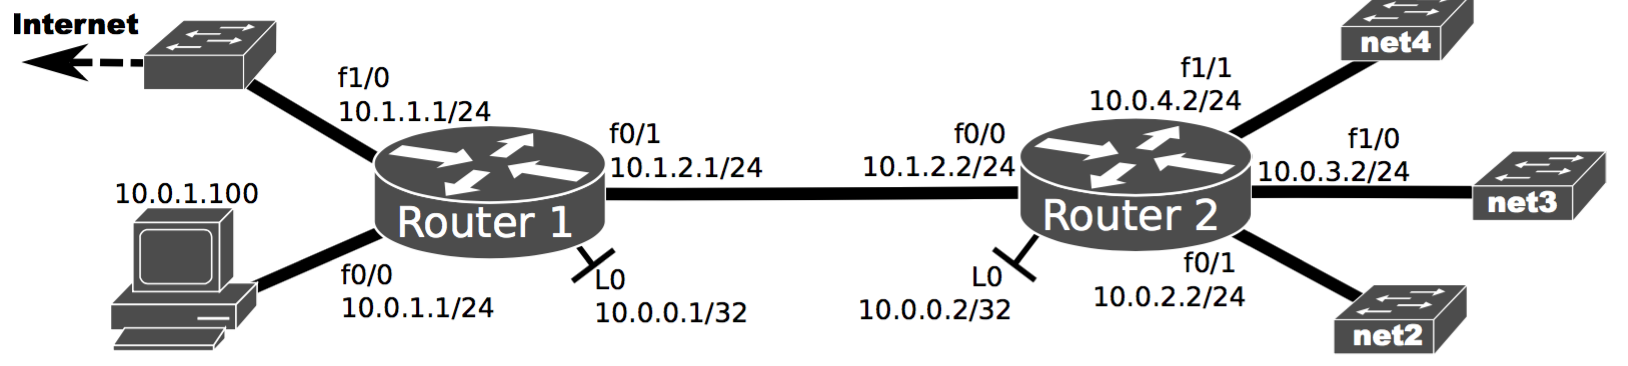
\includegraphics[width=150mm,scale=1]{imagens/mapa.png}
 \caption{Mapa de IP's}
 \label{fig:mapadeips}
\end{figure}

\begin{figure}[!htb]
\center
 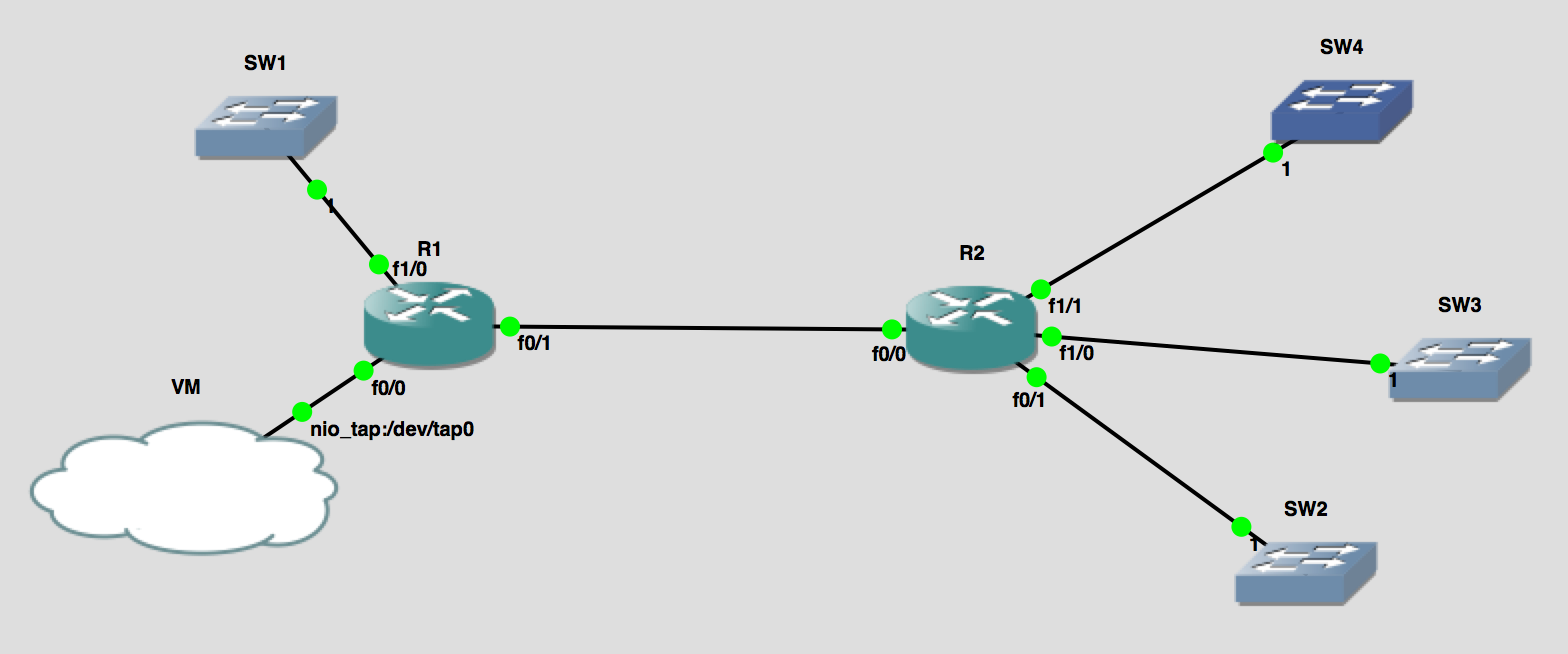
\includegraphics[width=150mm,scale=1]{imagens/gns_image.png}
 \caption{Mapa de IP's}
 \label{fig:mapadeips}
\end{figure}

\subsection{Implementação com Python}

\subsection{Apresentação de gráficos}

\newpage

\section{Conclusão}

O principal objetivo foi conseguido, queria-se fazer os 22 valores do trabalho para termos uma noção minimalista do que um Operador normalmente tem de ter e as várias possibilidades que podem ser feitas e soluções que podem ser desenvolvidas. 

Este trabalho serviu para meter em prática muita coisa que tinha sido falado na teórica e que ainda não se tinha tido oportunidade de se abordar na prática, sendo assim, o projeto foi divertido e interessante de ser realizado.

\end{document}